% https://ieeexplore.ieee.org/abstract/document/6248074 / aus anderer src => https://www.cs.toronto.edu/~urtasun/publications/geiger_et_al_cvpr12.pdf
% https://arxiv.org/abs/2504.16930
% https://arxiv.org/abs/2403.04965
% https://arxiv.org/abs/1512.02134 not used

\section{Dataset}
For the evaluation process or training, a dataset is required. A dataset contains a pair of stereo images and a ground-truth depth / disparity map. There are mainly two options for creating such a dataset, either in the real-world with stereo image sensors or computer-generated synthetic data.

Therefore, there are two essential ways to create such a dataset: either in the real-world using stereo image sensors, or using computer-generated synthetic data.

\subsection{Real-World approach}
Creating a real-world dataset requires substantial resources and time. Stereo sensors are required and must be calibrated. The environment needs to be carefully selected, especially with regard to lighting. Motion in the scenes is also a significant challenge. Since the KITTI dataset was captured from a vehicle, 3D sensing accuracy was therefore particularly important \cite{6248074}.

\subsection{Synthetic approach}
Creating a dataset in a synthetic environment offers the greatest possibility. This can save considerable time and resources, especially when specialized scenes are required. Furthermore, because the dataset is generated in a synthetic environment, the depth / disparity map can provide more accurate ground-truth, since the computation is not based on approximated values.

\subsection{Our Solution}
We decided to create our own computer-generated synthetic dataset for several reasons. First if we use an existing dataset, we have no control over the scene composition. If it's a real-world based dataset, it may not contain depth / disparity map or only an approximate one. It is also unclear whether the dataset has already been used in an existing training process. If so the evaluation could be biased.

Creating our own synthetic dataset could also provide greater possibilities for camera setups, if required in later training or evaluation. This would be much more difficult to achieve with a real-world camera setup.

As a render engine we used Blender. We set up a custom scene and a stereo rendering system. \\
In our initial approach, we generated the scene in a random, simple procedurally way figure \ref{fig:procedural_approach}. The limitations of this initial approach were the low complexity of the given primitives and the scene overall. Also the level of complexity within the distance / background was too low \cite{yan2026makesgoodsynthetictraining}. To address these issues in consideration with our very limited resources and time, the new scene, shown in figure \ref{fig:improved_approach}, consists of some specially selected objects with different surface characteristics. These objects were specifically positioned in the scene and in combination with the background, they provide different levels of surface characteristics on different distances.

\subsubsection{Generation}
Our stereo rendering system consists of three stages. The first stage is the camera initialization. To get the capability to render a large number of images, we created a procedural stereo camera system, shown in Figure \ref{fig:camera_initialization}. This system consists of two tasks. \\
\\
In the first task, we define multiple POIs for each Object of interest. These points of interest are used to orient the cameras towards the nearest POI. Second, we create camera paths around each object of interest. Cameras are later automatically placed along these paths by a script. The script then distributes a specified number of cameras evenly along the paths. \\
\\
The second stage is the stereo image rendering and the associated depth map generating within in Blender. This is done using another script that iterates over the pre-initialized cameras. For each camera, the script creates a temporary stereo camera configuration with randomly parameters within predefined bounds. Based on this configuration the stereo image pairs are rendered. In this process, the baseline and focal length are randomized. In addition, the depth map is generated for the left image (EXR format). \\
The lighting, objects and materials remain static throughout the entire creation process and are therefore not automatically randomized. \\
\\
The third stage consists of disparity map generation, which is a separate process outside of Blender. Therefore, a separate script is used to generate the corresponding disparity map (EXR format) for each sample. \\
\\
The following formula was used for this \cite{Wang-2024-stereodiffusion}: \\
$D(x,y)=\frac{fB}{Z(x,y)}$
\\
\\
Our dataset consists of four main objects. For each of these main objects, 1000 samples were generated. Each sample consists of a pair of stereo images with a resolution of 512$\times$512 pixels, along with the corresponding disparity map, depth map, and metadata. Due to the large amount of data, we decided to use JPG compression.

\subsubsection{Example}
Figure \ref{fig:dino_example} shows a sample of our dataset. \\
The stereo configuration parameters are as follows: \\
Baseline: 0.1 m \\
Focal Length: 38.4 mm \\

\begin{figure}[htpb]
    \centering
    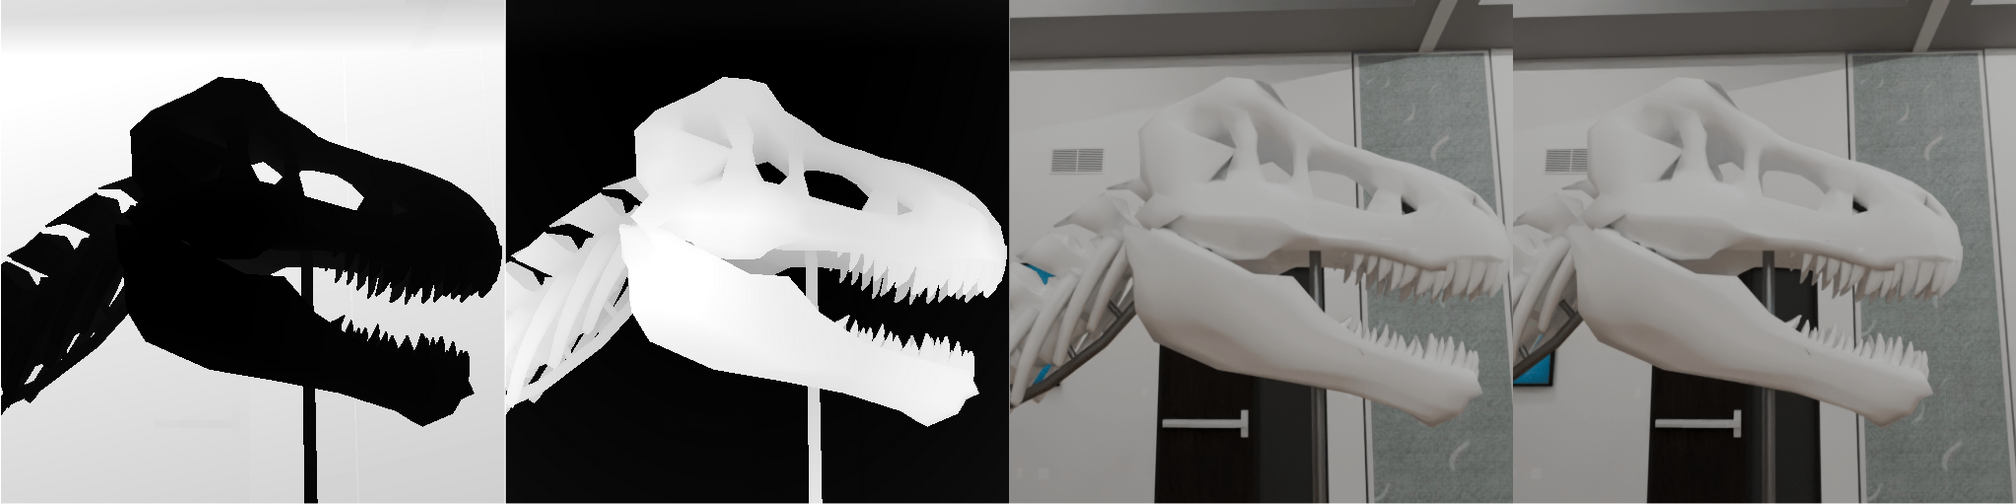
\includegraphics[width=1.0\linewidth]{figures/dino_example.png}
    \caption{Example sample - depth map, disparity map, left image, right image}
    \label{fig:dino_example}
\end{figure}

% left/right?